\section{Método dos Elementos Finitos (FEM)}\label{fem}
A presente seção busca introduzir alguns dos importantes conceitos referentes ao
método dos elementos finitos. Busca-se balancear a exposição de conceitos
fundamentais com uma maneira sintética de expor tais ideias de modo a ser
conciso e didático. Para mais informações refere-se a \cite{langtangen2017}
livro base onde a estrutura da presente seção foi baseada.

As equações diferenciais são as representações mais importantes de fenômenos
físicos. A descrição de taxas temporais ou de gradientes espaciais levam em
consideração a ideia do efeito que um pequeno diferencial em uma variável
independente (tempo, dimensão em $x$, $y$, ou $z$) tem em uma variável
dependente (temperatura, campo elétrico, magnético, tensão mecânica, etc.).

Tais equações podem ser classificadas em equações diferencias ordinárias (ODE)
quando se tem apenas funções de uma única variável e suas derivadas, ou em
equações diferencias parciais (PDE) quando se tem funções de várias variáveis e
suas derivadas parciais.

No geral, as ODE's lineares podem ser resolvidas analiticamente, isto é, é
possível obter sua solução em uma forma fechada (uma expressão matemática que
pode ser avaliada em um número finito de operações). Por outro lado, as PDE's
muitas vezes exigem procedimentos de solução mais complexos, fazendo uso de
expansões em séries, análises de similaridade e análises assintóticas. Uma grande
complicação de tais métodos é que em geral funcionam apenas para geometrias e
condições de contorno relativamente simplistas.

Como alternativa a tais métodos e através do avanço da capacidade computacional
os métodos numéricos alcançaram uma elevada relevância. O desenvolvimento de
\textit{softwares} comerciais permitiram que tais métodos fossem popularizados
entre usuários sem que estes precisem saber todos os detalhes da metodologia.
Porém, tais \textit{softwares} se especializaram em análises mais populares como
por exemplo cálculos de análises estruturais e da equação de calor. Dessa forma, casos mais
complicados onde se tem o acoplamento de situações relativamente incomuns (como
o acoplamento do transporte de massa e de energia) não são implementados.

Assim, justifica-se o desenvolvimento de um modelo através da metodologia dos
elementos finitos, uma das mais comuns metodologias de solução de PDE's e ODE's
através do uso de uma malha para representar domínios com geometrias complexas.
Para tanto, utilizar-se-á o pacote FEniCS da linguagem Python. Como o
desenvolvimento do modelo se dará desde a escolha do tipo de elemento, das
funções de forma, nós de integração entre outros, é necessário revisar os
conceitos fundamentais necessários para a implementação do modelo.

	\subsection{Métodos de aproximação de funções}
	A metodologia por trás do FEM, é uma formulação já estabelecida que permite
  fazer a aproximação de funções de uma maneira sistemática através de funções
  de forma sobre uma malha. Tal metodologia é conhecida como o Método de Galerkin. Existem
  inúmeras variações de tal metodologia, com alterações pontuais, recebendo
  nomes distintos. No presente trabalho, apresentaremos e utilizaremos a
  metodologia de Galerkin.

  Antes de introduzir a metodologia de Galerkin para a obtenção de soluções
  numéricas de equações diferenciais, iniciaremos e definiremos objetos
  matemáticos a partir da aproximação de Galerkin para funções (de fato,
  aproximação de vetores). Isso tornará a metodologia mais palpável.

  \subsection{Aproximação de Galerkin}
  Para ilustrar a metodologia utilizaremos a aproximação de uma equação
  trivial: 
  \begin{equation}
  \uvec = \vvec
  \end{equation}
  Tal equação representa a busca pela melhor aproximação do vetor $\vvec$ 
  Existem duas abordagens motivadas por conceitos da álgebra
  linear que nos permitem formalizar algoritmos para resolver essa tarefa, são
  elas a metodologia dos mínimos quadrados e a metodologia de projeção. Tais
  metodologias são ilustradas nas Definições \ref{def:minqua} e \ref{def:metproj} 

  \begin{Definition}{Metodologia dos Mínimos Quadrados}{minqua}
  A melhor aproximação de um vetor, $\vvec$ se dá quando o vetor erro, isto é a
  diferença entre o vetor $\vvec$ e a aproximação $\uvec$, possui a menor norma
  (a partir da métrica definida no espaço vetorial em questão) possível.
  \end{Definition}

  \begin{Definition}{Metodologia da Projeção}{metproj}
  A melhor aproximação de um vetor, $\vvec$, se dá quando seu erro, o vetor $\evec =
  \vvec - \uvec$ é perpendicular (o termo correto seria ortogonal) ao
  subspaço ao qual o vetor $\vvec$ reside.
  \end{Definition}
  A metodologia proposta na Definição \ref{def:minqua} é bastante intuitiva,
  porém a metodologia da Projeção pode ser mais complicada de se visualizar.
  Para tanto, uma forma de visualizar se encontra na Figura \ref{fig:2dvecs}.
  Observe que a aproximação da figura representa a aproximação de dois vetores
  existentes em um espaço Euclidiano representado em coordenadas Cartesianas, o
  que poderá ser generalizado para vetores definidos em espaços de maiores, ou
  ainda infinitas dimensões. Nesse contexto, como funções são vetores, pode-se
  garantir que ambas metodologias acima definidas também resultarão em
  metodologias de aproximação de funções (que são vetores, afinal).

  \begin{figure}[ht]
	\centering
	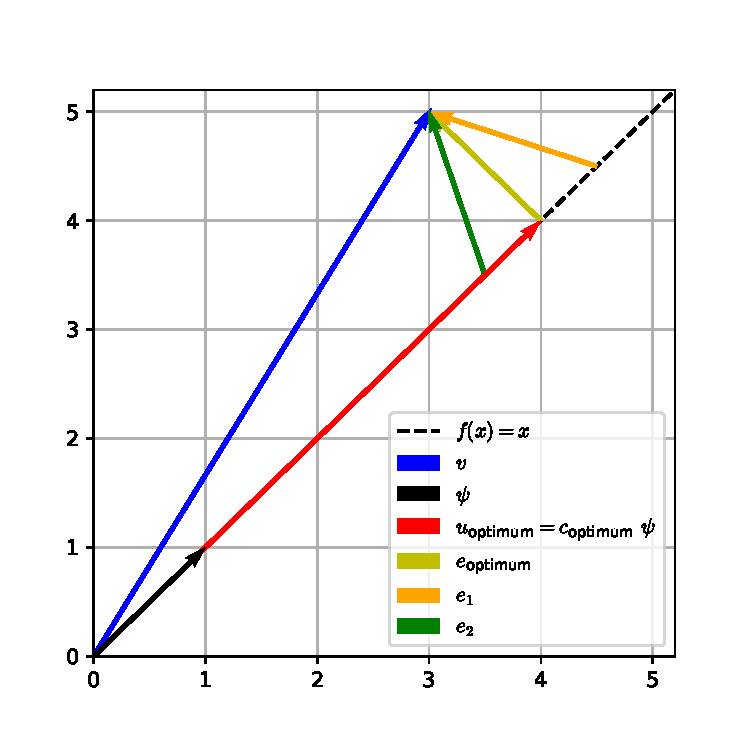
\includegraphics[width=\linewidth]{./figures/2dvectors.pdf}
	\caption{Representação da aproximação de vetores bidimensionais em coordenadas
    Cartesianas.  \label{fig:2dvecs}}
  \end{figure}

  É evidente que a melhor aproximação $\uvec_{optimum}$ resulta no erro de menor
  norma Euclidiana (comprimento do vetor, seguindo a definição de uma norma em um espaço
  vetorial Euclidiano), entretanto observe também que o erro ótimo,
  $evec_{optimum}$ é perpendicular a reta onde reside o vetor $\uvec$ que estamos
  tentando aproximar. Lembrando-se da Geometria Analítica, quando dois vetores
  são perpendiculares seu produto interno é nulo.

  Assim, a metodologia para obter a melhor aproximação de um vetor $\fvec$
  pertencente ao espaço vetorial $V=\spn \{\bm{\mathrm{\psi_0}},
      \bm{\mathrm{\psi_1}}, \dots, \bm{\mathrm{\psi_N}} \}$ (onde
          $\bm{\mathrm{\psi_i}}$ é o i-ésimo vetor base do espaço vetorial $V$,
            isto é, o conjunto de vetores linearmente independentes com os quais
            se pode obter através de combinações lineares todos os vetores de $V$) através do método da Projeção se
  baseará na minimização da seguinte equação vetorial:

  $$ \evec \cdot \vvec = 0$$
  
  Através dessa equação obtém-se um sistema de equações lineares que permite
  encontrar os coeficientes da combinação linear que define a melhor aproximação
  do vetor $\vvec$ no espaço vetorial $V$. O russo Boris Galerkin usou o mesmo
  princípio para obter a solução de equações diferenciais CITAÇÃO, definindo o
  método de Galerkin.
  
	\subsection{Funções de forma}
	Como visto, anteriormente nos exemplos de vetores de duas dimensões no espaço
  Euclidiano, as aproximações de determinado vetor podem ser representadas
  através de combinações lineares de coeficientes e os vetores bases que definem
  o espaço vetorial. O que as métodologias de aproximação fornecem, são
  algoritmos que permitem encontrar o conjunto de coeficientes que formam a
  combinação linear dos vetores base cujo erro é o menor possível (dado uma
  certa métrica), segundo a Definição \ref{def:minqua} ou que o erro seja
  ortogonal ao subespaço ao qual o vetor a ser aproximado reside, segundo a
  Definição \ref{def:metproj}.

  Assim, é evidente que a escolha dos vetores base é uma escolha primordial para
  que o processo de aproximação seja o mais prático possível. Dentre as várias
  possibilidades, é comum a busca por vetores ortogonais e isso pode ser
  mostrado pelo apelo que certas funções ortogonais apresentam como as funções
  trigonométricas seno e cosseno que são as bases das aproximações de Fourier.

  No caso de tais funções trigonométricas seu domínio é o mesmo que todo o
  domínio ao qual a função a ser aproximada se estende, porém, uma estratégia
  que se pode utilizar é o uso de funções base com suporte compacto, isto é,
  funções que são não nulas apenas em uma porção do domínio, e que é zero em
  todo o resto do domínio, essas funções bases são as funções de elemento finito.

  Tais funções são excelentes motivações para a divisão do domínio em uma malha,
  pois em cada elemento de determinada malha tem-se funções de forma que são não
  nulas nessa região do domínio. A vantagem é que se pode definir domínios
  complexos de uma maneira sistemática onde a convergência é obtida conforme a
  malha se torna mais refinada, isto é, com menores elementos além de se obter,
  durante a resolução, matrizes que são positivas definidas, o que facilita a
  resolução numérica.

    \subsubsection{Malha}
    A malha é uma partição do domínio em elementos cuja intersecção é nula e
    cuja união resulta exatamente no domínio. O conceito mais generalizado de um
    elemento finito é apresentado na Definição \ref{def:elemento}.

    \begin{Definition}{Definição Geral de Elemento Finito}{elemento}
      \begin{itemize}
        \item Um elemento finito é uma célula em um sistema de coordenadas
      locais de referência cujos limites são chamados de vértices.

        \item Em cada célula se define um conjunto de funções base do tipo de elementos
      finitos e um conjunto de graus de liberdade, isto é, quantidades que se
      busca calcular (por exemplo, a temperatura em determinado ponto ao resolver
      a equação de calor).

     
        \item Finalmente define-se um mapa entre os graus de liberdade locais (de dentro
      do elemento) e os globais (definidos em todo domínio). Tal mapa serve para
      organizar os resultados obtidos após o cálculo. Além disso, define-se um
      mapa geométrico entre a célula e o domínio físico.
      \end{itemize}
      \end{Definition}

    A princípio pode-se parecer que tais definições acabem tornando o método
    apenas mais complexo e abstrato. Porém, tal abstração garante que agora a
    metodologia de resolução no elemento seja feita individualmente elemento a
    elemento (usando o mesmo procedimento, pois usa-se o mesmo elemento de
    coordenadas de referência) sem considerar as especificidades
    referentes a geometria. Após o cálculo se realiza o processo de
    \textit{assembly} onde se obtém os graus de liberdade em todo domínio.

    Uma vez definido a malha e os elementos a resolução do sistema de equações
    pode ser montado a partir da forma variacional do problema. A seção seguinte
    traz o conceito de forma variacional.

    \subsection{Forma variacional}
    
    \subsection{Integração numérica}
    Conforme observado 
